\section{Signes et communication}

\begin{frame}{Importance des signes}
  \begin{itemize}
    \item Sous l’eau, on ne parle pas : les \textbf{signes manuels} sont le seul moyen sûr de communication.
    \item Ils doivent être \textbf{amples, clairs et sans ambiguïté}.
    \item Permettent de transmettre rapidement :
          \begin{itemize}
            \item un \textbf{problème},
            \item une \textbf{information},
            \item un \textbf{ordre de sécurité}.
          \end{itemize}
  \end{itemize}
\end{frame}

\begin{frame}{Signes de base (exemples)}
  \centering
  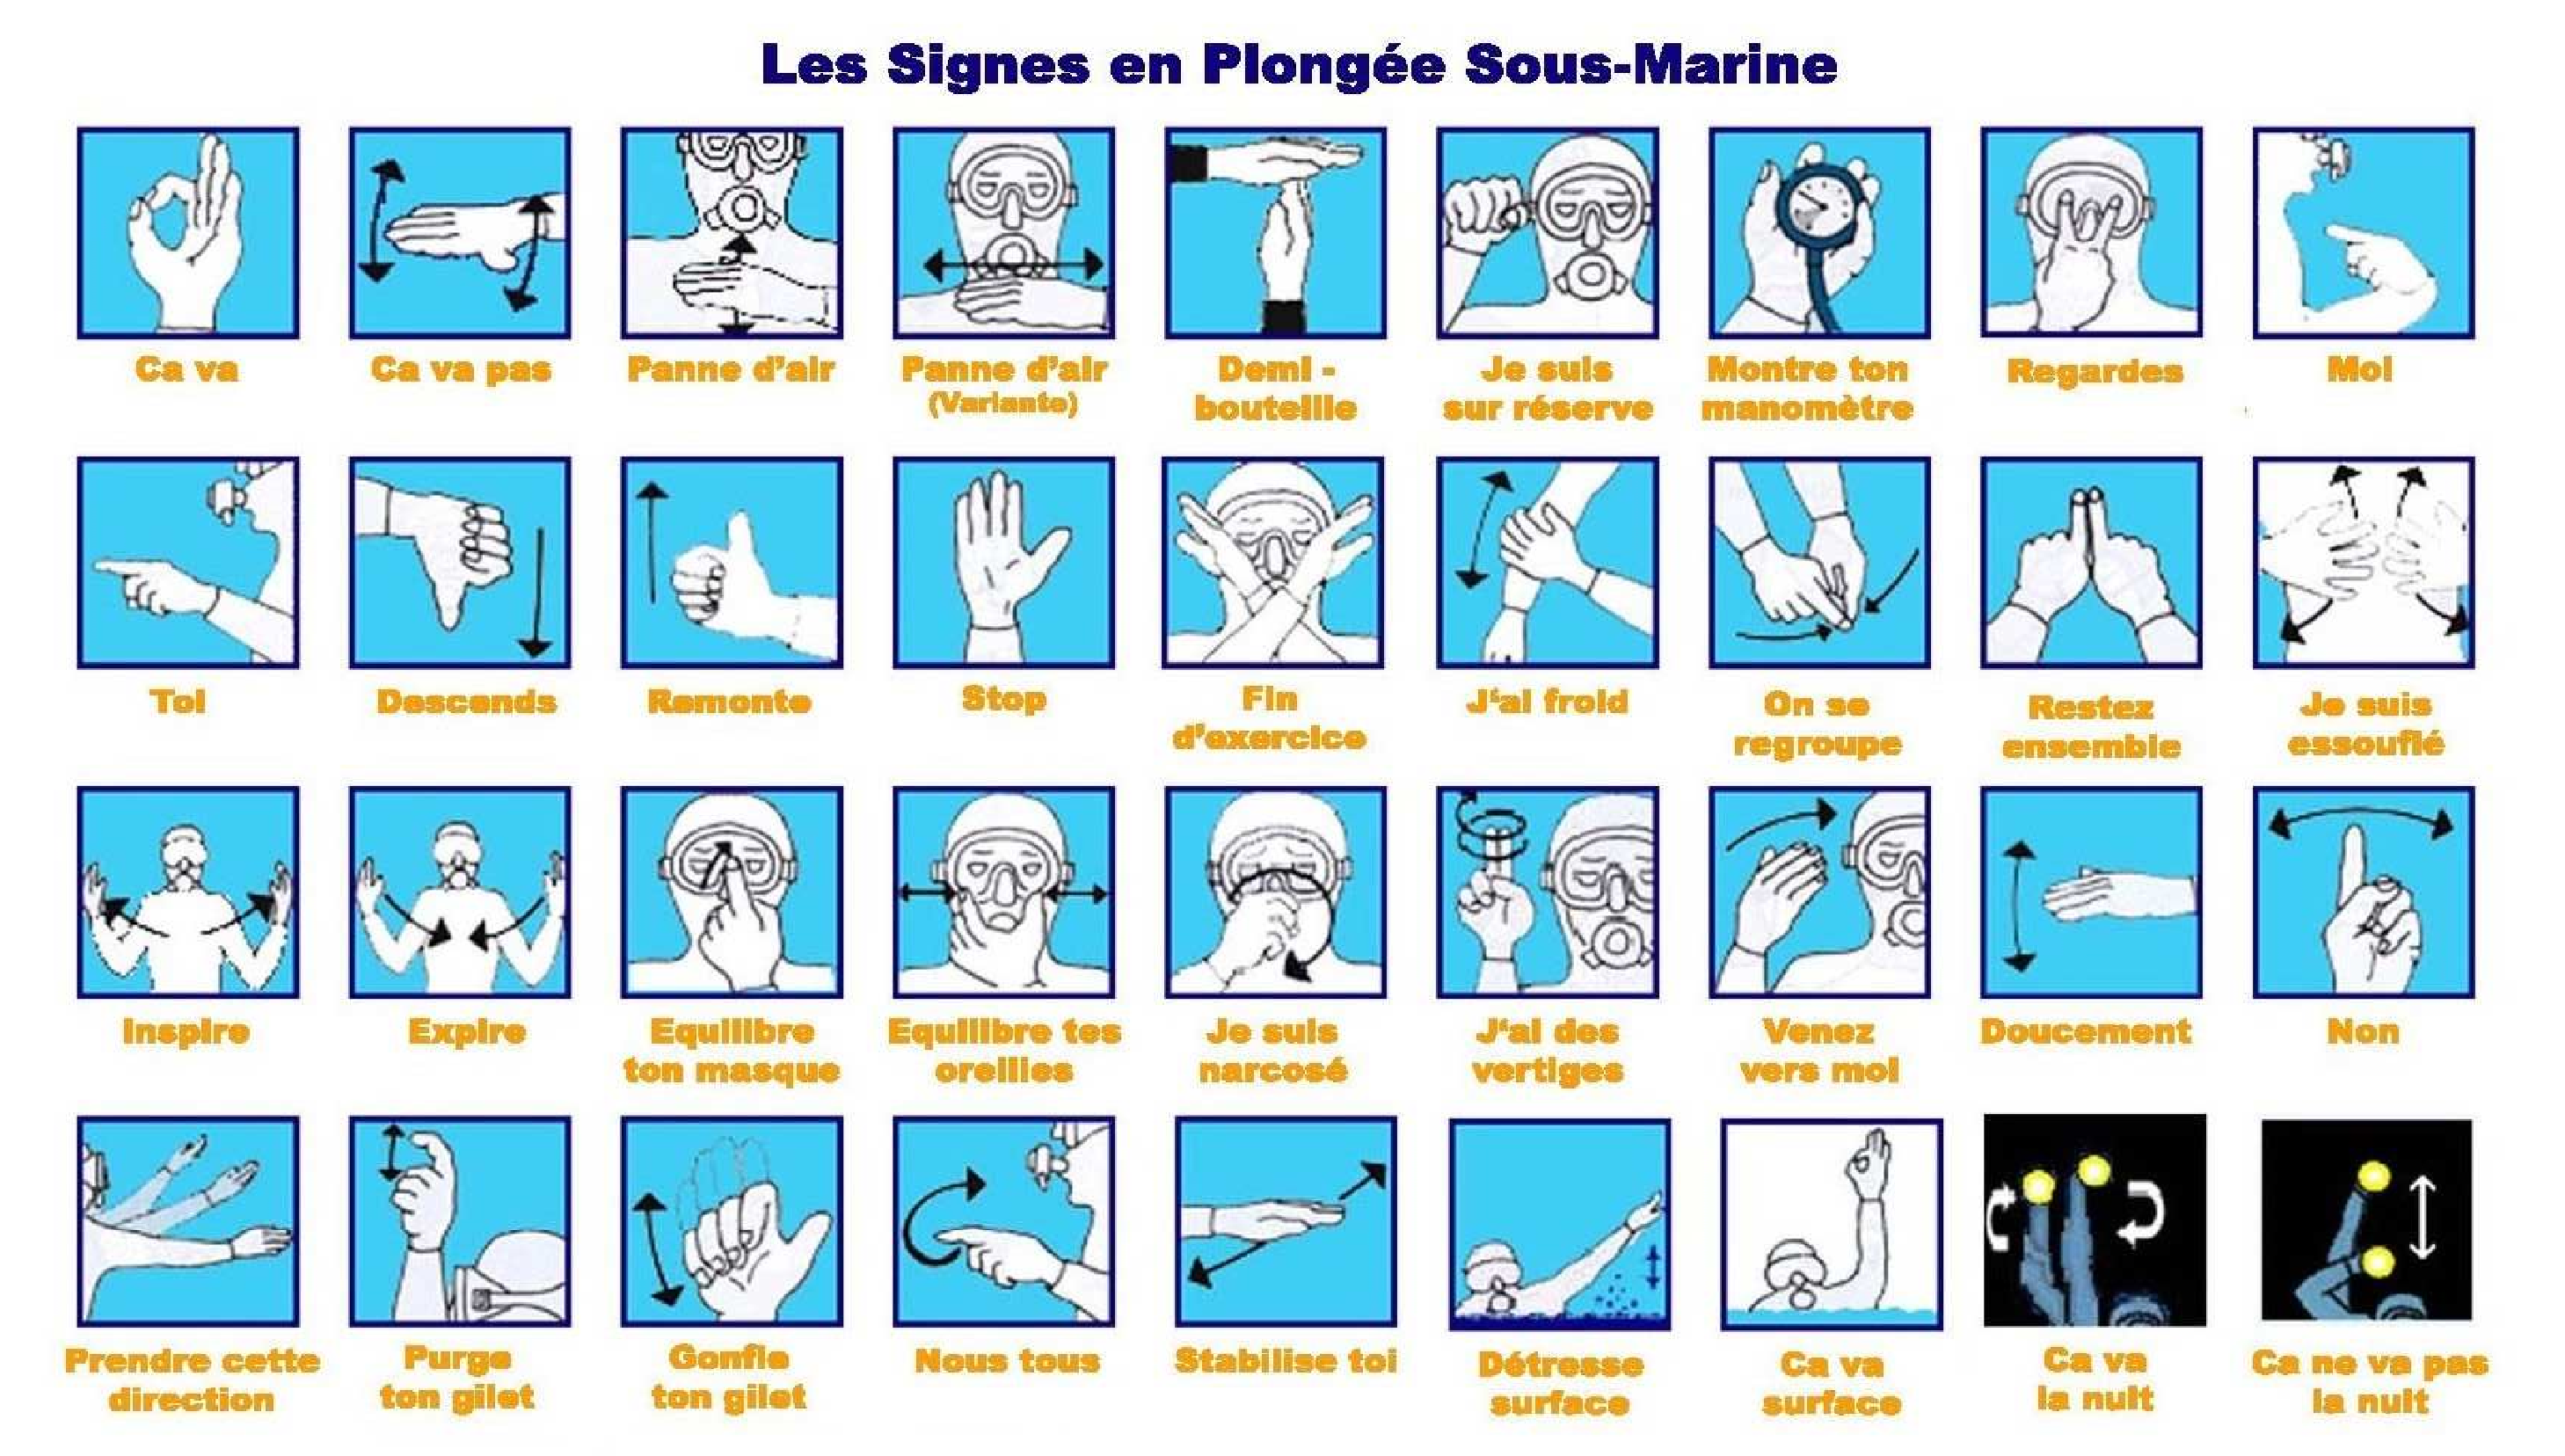
\includegraphics[width=0.79\textwidth]{images/signes_communication}
\end{frame}
